%
% 6.006 problem set 5 solutions template
%
\documentclass[12pt,twoside]{article}

\usepackage{amsmath}
\usepackage{color}
\usepackage{tikz}

\input{macros}

\setlength{\oddsidemargin}{0pt}
\setlength{\evensidemargin}{0pt}
\setlength{\textwidth}{6.5in}
\setlength{\topmargin}{0in}
\setlength{\textheight}{8.5in}

\newcommand{\theproblemsetnum}{5}
\newcommand{\releasedate}{Thursday, November 12, 2015}
\newcommand{\partaduedate}{Tuesday, November 24, 2015}
\newcommand{\tabUnit}{3ex}
\newcommand{\tabT}{\hspace*{\tabUnit}}

\title{6.006 PSET 5}

\begin{document}

\handout{Problem Set \theproblemsetnum}{Thursday, November 12, 2015}

\textbf{All parts are due {\bf \partaduedate} at {\bf 11:59PM}}.

\setlength{\parindent}{0pt}

\medskip

\hrulefill

\medskip

{\bf Name:} Budmonde Duinkharjav

\medskip

{\bf Collaborators:} Kevin Liu, Danny Tang

\medskip

\hrulefill

%%%%%%%%%%%%%%%%%%%%%%%%%%%%%%%%%%%%%%%%%%%%%%%%%%%%%
% See below for common and useful latex constructs. %
%%%%%%%%%%%%%%%%%%%%%%%%%%%%%%%%%%%%%%%%%%%%%%%%%%%%%

% Some useful commands:
%$f(x) = \Theta(x)$
%$T(x, y) \leq \log(x) + 2^y + \binom{2n}{n}$
% {\tt code\_function}


% You can create unnumbered lists as follows:
%\begin{itemize}
%    \item First item in a list 
%        \begin{itemize}
%            \item First item in a list 
%                \begin{itemize}
%                    \item First item in a list 
%                    \item Second item in a list 
%                \end{itemize}
%            \item Second item in a list 
%        \end{itemize}
%    \item Second item in a list 
%\end{itemize}

% You can create numbered lists as follows:
%\begin{enumerate}
%    \item First item in a list 
%    \item Second item in a list 
%    \item Third item in a list
%\end{enumerate}

% You can write aligned equations as follows:
%\begin{align} 
%    \begin{split}
%        (x+y)^3 &= (x+y)^2(x+y) \\
%                &= (x^2+2xy+y^2)(x+y) \\
%                &= (x^3+2x^2y+xy^2) + (x^2y+2xy^2+y^3) \\
%                &= x^3+3x^2y+3xy^2+y^3
%    \end{split}                                 
%\end{align}

% You can create grids/matrices as follows:
%\begin{align}
%    A = 
%    \begin{bmatrix}
%        A_{11} & A_{21} \\
%        A_{21} & A_{22}
%    \end{bmatrix}
%\end{align}

\begin{problems}

\section*{Part A}

\problem % Problem 1
To solve this problem, we will implement the same algorithm as in \emph{Bellman-Ford}. I.e. we will relax every single node without any preference $M$ times. We justify this algorithm by:
\begin{enumerate}
\item \emph{Bellman-Ford} also says that given that there are no negative cycles in the graph, by the $i$th iteration, we will have found the shortest path to a node which is $i$ edges away from the source. If we reverse the problem by saying that we start with $0$ points and must not reach $M$ points and make all $p(x, y)$s positive, we will still be solving the same problem. Since here, we have no negative edges, we know that we can't have negative cycles.
\item We are given that any damage Ben takes is a non-zero integer amount and that $M$ is an integer. Therefore we know that Ben can reach coordinates which are at most $M$ away, with best case being that every coordinates he goes to has $p(x, y)$ of $1$.
\end{enumerate}
From here, we see that if we haven't found a valid path from the source to the target after $M$ iterations of \emph{Bellman-Ford}, Ben cannot escape. Since we are running \emph{Bellman-Ford} $M$ times and that $E=O(V)$, we know that the runtime is $O(MV)$ which is $O(Mn^2)$ in terms of $n$.


\problem % Problem 2
To solve this problem we approach this by creating a procedure which resembles \emph{BFS}, each procedure running a \emph{Dijsktra} algorithm. Before we begin describing the algorithm, we note that we adjust the problem such that all edge weights are positive and Ben starts from $0$ points and is avoiding overshooting the value of $M$.\\

First, we take the source node and run \emph{Dijkstra} on it marking all nodes which have a health pack in it which is also less than $M$ distance away from the source. Let's call the list of these nodes, {\tt reacheable\_nodes}. After we are done with this procedure, we push all the elements of this list into a queue, {\tt queue} in no particular order. We treat {\tt queue} the same way we treat it to run a \emph{BFS} algorithm: From this point on, we pop the first element of the queue and run \emph{Dijkstra} on it to find the next set of {\tt reacheable\_nodes} and push them to the end of {\tt queue}. We will halt the entire procedure if we either reach the target node, or {\tt queue} empties. In the case {\tt queue} empties, we will return that 'Ben's trapped for good' but if we reach the target node, we will return a path between all used health packs in the order they are used along with the final \emph{Dijkstra} that reached the target node.\\

The runtime of this algorithm is \emph{BFS} with every node expansion taking \emph{Dijkstra}'s runtime. As \emph{BFS} expands $O(K)$ nodes and each expansion takes $O(V \log V)$ since $E = O(V)$, the total runtime is $O(K V \log V)$ or $O(K n^2 \log n)$ in terms of $n$ since $V = n^2$.


\section*{Part B}
\problem % Problem 3
\begin{problemparts}

\problempart % Problem 3a

\textbf{Proof of Claim 1.}
$r = l' \mod a = l \mod a$ and $l' > l$ implies that there exist some integers $m > n$ such that $l' = a m + r$ and $l = a n + r$. We know that $l$ is a whimsical number. Then, we see that $l' = a (m - n) + l$ which is clearly a whimsical number. Here we can also see how this statement would become false in the case $m < n$. We will be using this argument for the next part.

\textbf{Proof of Claim 2.}
Let's say for a given $l$ and $a$, $x_r$ exits. Then, we see that $l \mod a = x_r \mod a$. By \textbf{Claim 1}, we know that if $l \geq x_r$, $l$ must be a whimsical number. Then, let's say that for the given $l$ and $a$, $x_r$ did not exist but $l$ was a whimsical number. We can express $l = a m + r$ for some integer $m$. But then there exists an $x_r = l$. By contradiction this condition is proven. Lastly, consider the case where $l$ is a whimsical number, and $x_r > l$. But then since $l$ is a whimsical number $x_r$ is no longer the smallest integer such that $x_r \mod a = r$. $l$ is. By contradition this condition is also false. Therefore this claim is true.

\problempart % Problem 3b
We implement the alogorithm as follows. For the smallest element  $a_{min} \in A$, we create vertices, labeled $\{0,1,2...a-1\}$. Then, for each $a \in A$, we create an edge connecting node $i$ with node $(i+a) \mod a_{min}$.
\begin{figure}[!h]
\centering
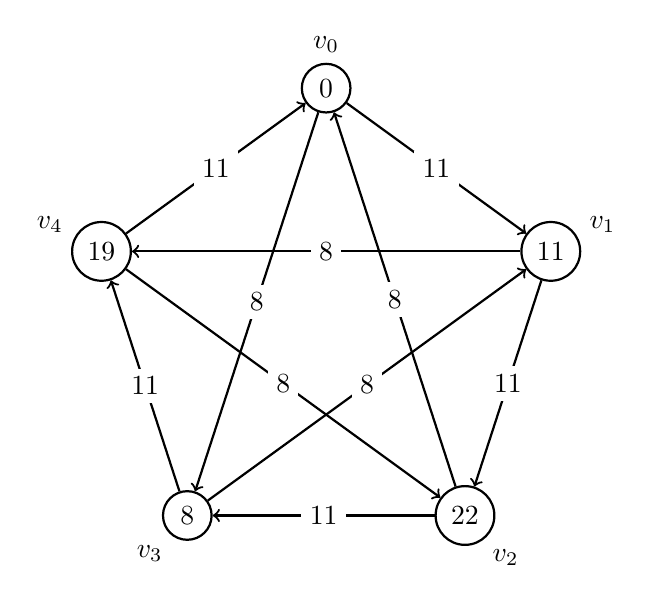
\begin{tikzpicture}[
   vertex/.style={circle,draw,thick},
   edge/.style={draw=black,thick, ->}]
   % replace the ?'s below with your shortest path distances for nodes v1, v2, v3, v4, respectively
   % may cause errors if you break it into multiple lines
   \foreach \r/\dist in {{0/0},{1/11},{2/22},{3/8},{4/19}}
      \node[vertex,label={{90-\r*72}:$v_{\r}$}] (v\r) at ({90-\r*72}:3) {\dist};
   % add edges to the list; format: {from/to/weight}
   % may cause errors if you break it into multiple lines
   \foreach \from/\to/\weight in {{v0/v1/11},{v0/v3/8},{v1/v2/11},{v1/v4/8},{v2/v3/11},{v2/v0/8},{v3/v4/11},{v3/v1/8},{v4/v0/11},{v4/v2/8}}
      \draw[edge] (\from) edge node[fill=white,rectangle, inner sep=3pt]{\weight} (\to);
\end{tikzpicture}
\end{figure}
 
\problempart  % Problem 3c
With the graph set up as such, we simply need to find the values $x_r$ of each node, as computed when solving the first part of this part. We do so by implementing a \emph{Dijkstra} algorithm starting from node $0$ until we read all nodes. Having found all $x_r$s we may now use \textbf{Claim 2} from \emph{part (a)} to show that we can find whether an input $l$ is whimsical or not by computing $r = l \mod a_{min}$ and checking whether $x_r$ for the corresponding $r$ exists and whether this $x_r \leq l$. If either condition fails, $l$ would not be a whimsical number.\\

Runtime for preprocessing includes creating the graph, which takes $O(kM)$ time since there are $k$ elements in $A$ and $a_{min} \leq M$. Then, running \emph{Dijkstra} takes $O(E \log V)$ or $O(kM \log M) = O(kM \log kM)$.

As we are storing $r, x_r$ pairs in a dictionary, access time with $r$ as key will take $O(1)$ time and all computations are arithmetic and logic operations on integers without any loops, the overall runtime is still $O(1)$.

\problempart \emph{Submit your implemented python script.}  % Problem 3d

\end{problemparts}
\end{problems}
\end{document}



























